\newpage
\section{Backpropagation and Neural Networks}
\subsection{Backpropagation}

\begin{align*}
    s&=f(x;W)=Wx &\text{scores function}\\
    L_i&=\sum_{j\ne y_i}\max (0, s_j-s_{y_i}+1) &\text{SVM loss}\\
    L&=\frac{1}{N}\sum_{i=1}^N L_i+\sum_k W_k^2 &\text{data loss + regularization}
\end{align*}
we want $\nabla_W L$

\subsubsection{Computational graphs}
\begin{figure}[!htb]
    \centering
    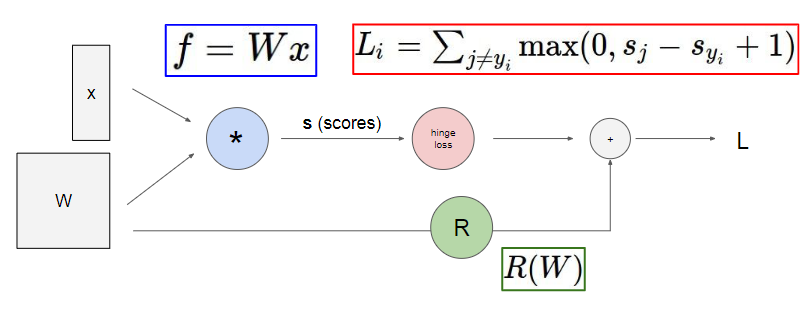
\includegraphics[width=0.42\textwidth]{pic/Lec4/Computational graphs}
    \caption{Computational graphs}
\end{figure}

节点是函数操作, 边是数据. 

\subsubsection{Backpropagation}
链式法则, 反向传播, 可以把常用的复杂计算合成一块. 
\paragraph{Patterns in backward flow}
\begin{enumerate}
    \item \textbf{add} gate: gradient distributor
    \item \textbf{max} gate: gradient router (路由器, 导向?)
    \item \textbf{mul} gate: gradient switcher
\end{enumerate}

Gradients add at branches (梯度在分支中相加)

\paragraph{Gradients for vectorized code} 求导变成求 Jacobian matrix
\subsubsection{Summary}
\begin{itemize}
    \item backpropagation 拆分求导
    \item forward 计算答案与梯度所需中间数
    \item backward 应用链式规则来计算损失函数相对于输入的梯度
\end{itemize}

\subsection{Neural Networks}
without the brain stuff

层的抽象具有良好的特性,它允许我们使用高效的矢量化代码. 

\textbf{Biological Neurons}:
\begin{enumerate}
    \item Many different types
    \item Dendrites can perform complex non-linear computations
    \item Synapses are not a single weight but a complex non-linear dynamical system
    \item Rate code may not be adequate
\end{enumerate}